\section{Umsetzung}
\subsection{Softwarearchitektur}
     Das Projekt gliedert sich grob in zwei Teile: Der erste Teil ist eine Java-Anwendung, die Berechnungen koordiniert, Benutzer-Interaktion händelt und Informationen
     (auch grafisch) aufbereitet. Der zweite Teil ist eine Perl-basierte Berechnungsanwendung (polymake~\cite{polymake}), an die Berechnungsaufträge ausgelagert werden.
     Eine grobe Übersicht über die Gesamtarchitektur kann in Abbildung~\ref{fig:architecture} gefunden werden.
     Die wichtigsten Bestandteile der Java-Anwendung sind folgende: (1) Repräsentation von geometrischen Objekten, wie Quaternionen, Symmetrien,
     Fundamentalbereichen, Schlegeldiagrammen und weiteren Objekten (siehe Paket \texttt{geometry}); (2) Verwaltung von Berechnungsaufträgen, Verteilung von Informationen innerhalb
     der Applikation und Fehlerbehandlung (siehe Paket \texttt{util}); (3) Reaktion auf Benutzereingaben, grafische Repräsentation der Berechnungsergebnisse (siehe Paket \texttt{gui}).

     \begin{figure}[tbh]
            \centering
            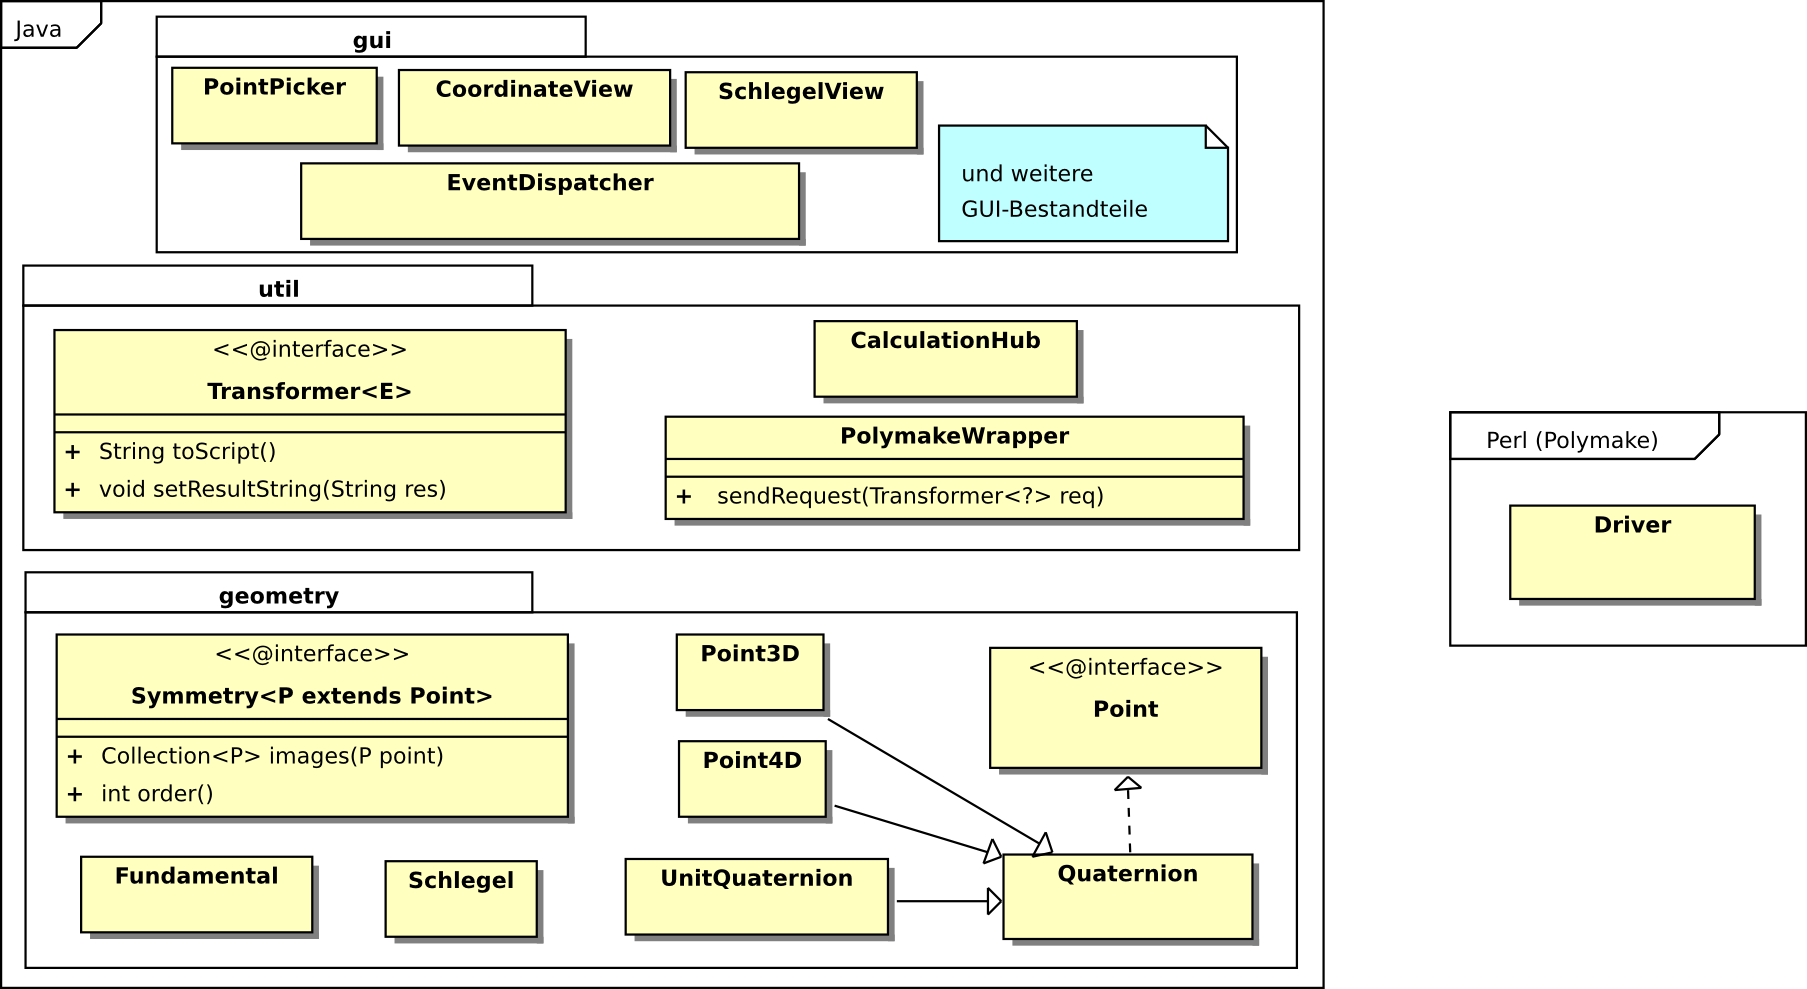
\includegraphics[width=0.85\textwidth]{img/architecture}
            \caption{Grobübersicht über die Architektur des Projekts\label{fig:architecture}}
        \end{figure}

    Dabei zeichnet sich das Projekt durch folgende Eigenschaften aus:
    \begin{itemize}
        \item Pipeline-artiger Informationsfluss (siehe~\ref{ssec:flow})
        \item Lose Kopplung durch Eventsystem (siehe~\ref{ssec:event})
        \item Aufbereitung der Daten durch GUI (siehe~\ref{ssec:gui})
    \end{itemize}
    \noindent Dabei wird folgende Entwurfsidee verfolgt: Polymake wird als externes Spezialrechenprogramm benutzt und mittels I/O mit Berechnungsaufträgen beliefert.
    Diese Berechnungsaufträge werden ad-hoc als Reaktion von Benutzereingaben (z.B. Anzeige einer 3D-Punktmenge) seitens der Java-Applikation erstellt und intern als
    Objekte repräsentiert. Da die Berechnungen von Polymake verschieden lange dauern, wird ein Ereignissystem (Event-basiertes System) umgesetzt, das an Berechnungsergebnissen
    interessierte Komponenten mittels Events von diesen informiert. Letztendlich wird die grafische Benutzeroberfläche mit den Resultaten der Berechnungen bestückt und
    geeignet angezeigt. Hierbei werden die Punktmengen als interaktiv durch die Maus drehbare Polytope angezeigt.

    \subsubsection{Verwendete Softwarehilfsmittel}
       \begin{description}
           \item [jReality]
                ~\cite{jreality} ist eine Bibliothek zum Erzeugen von Programmen mit Echtzeit-3D-Computergrafiken. Wir verwenden jReality innerhalb von Java-Swing Oberflächen zur Anzeige von Polytopen.
           \item [Polymake]
           	~\cite{polymake} ist ein Werkzeug um Berechnungen mit konvexen Polytopen (z.B. das Berechnen von konvexen Hüllen) auszuführen. Es wird entweder als Kommandozeilenanwendung oder online benutzt.
           \item [Maven]
                ~\cite{maven} ist ein Build-Tool und erlaubt das einfache Kompilieren von Java-Projekten und automatisierte Beschaffen von Abhängigkeiten.
           \item [JUnit]
                ~\cite{jUnit} ist ein Framework zum Testen von Java-Anwendungen mittels Unit-Tests. Mit den Tests kann nach jeder Änderung oder Neuerung automatisiert getestet werden, ob Methoden fehlerfrei funktionieren und das gewünschte Resultat liefern.
        \end{description}

    \subsubsection{Informationsfluss\label{ssec:flow}}
        \begin{figure}[tbh]
            \centering
            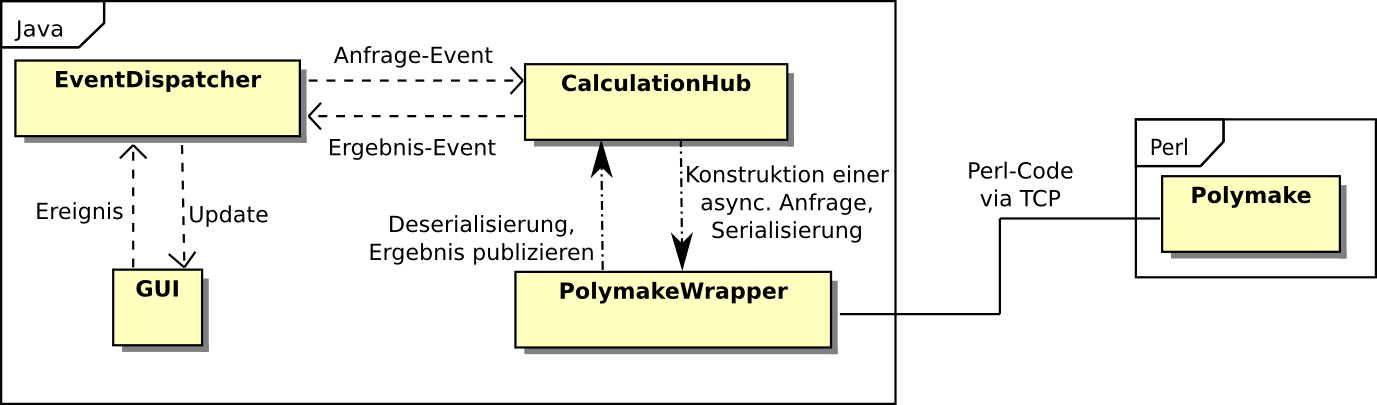
\includegraphics[width=0.85\textwidth]{img/flow}
            \caption{Informationsfluss zwischen den Komponenten
                      {\scriptsize(gestrichelt: sync. Methodenaufruf, punkt-strich: async. Methodenaufruf, durchgezogen: TCP-Nachricht}\label{fig:flow}}
        \end{figure}

        \noindent Die Eingabeinformationen der Anwendung passieren mehrere Berechnungsschritte nacheinander und beschreiben, wie in Abbildung~\ref{fig:flow} zu sehen, eine Pipeline-artige Struktur.
        Es werden über die grafische Oberfläche durch den Benutzer Anfangsinformationen vorgegeben (z.B. Koordinaten eines Punktes, Auswahl einer Symmetriegruppe)
        und damit mittels eines Events eine Berechnung gestartet. Hierbei passieren die resultieren Berechnungsaufträge einige interne Stationen der Java-Applikation:
        Eine Zentralinstanz, der \texttt{CalculationHub}, nimmt die Berechnungsanfrage zur Kenntnis und merkt sich diese noch offene Anfrage zur späteren Beantwortung.
        Zeitgleich wird die Anfrage mittels eines Abstraktionsobjektes (des \texttt{Polymakewrapper}s) an die laufende \texttt{polymake}-Instanz geschickt.
        Erreicht eine Antwort via I/O die Java-Applikation, so ordnet diese der \texttt{CalculationHub} der korrekten ursprünglichen Anfrage zu und informiert mittels Event alle
        interessierten Komponenten, dass ein Berechnungsergebnis vorliegt.
        Die GUI empfängt dann diese Informationen, bereitet sie auf und zeigt sie an.

    \subsubsection{Eventssystem\label{ssec:event}}
        \begin{figure}[bht]
            \centering
            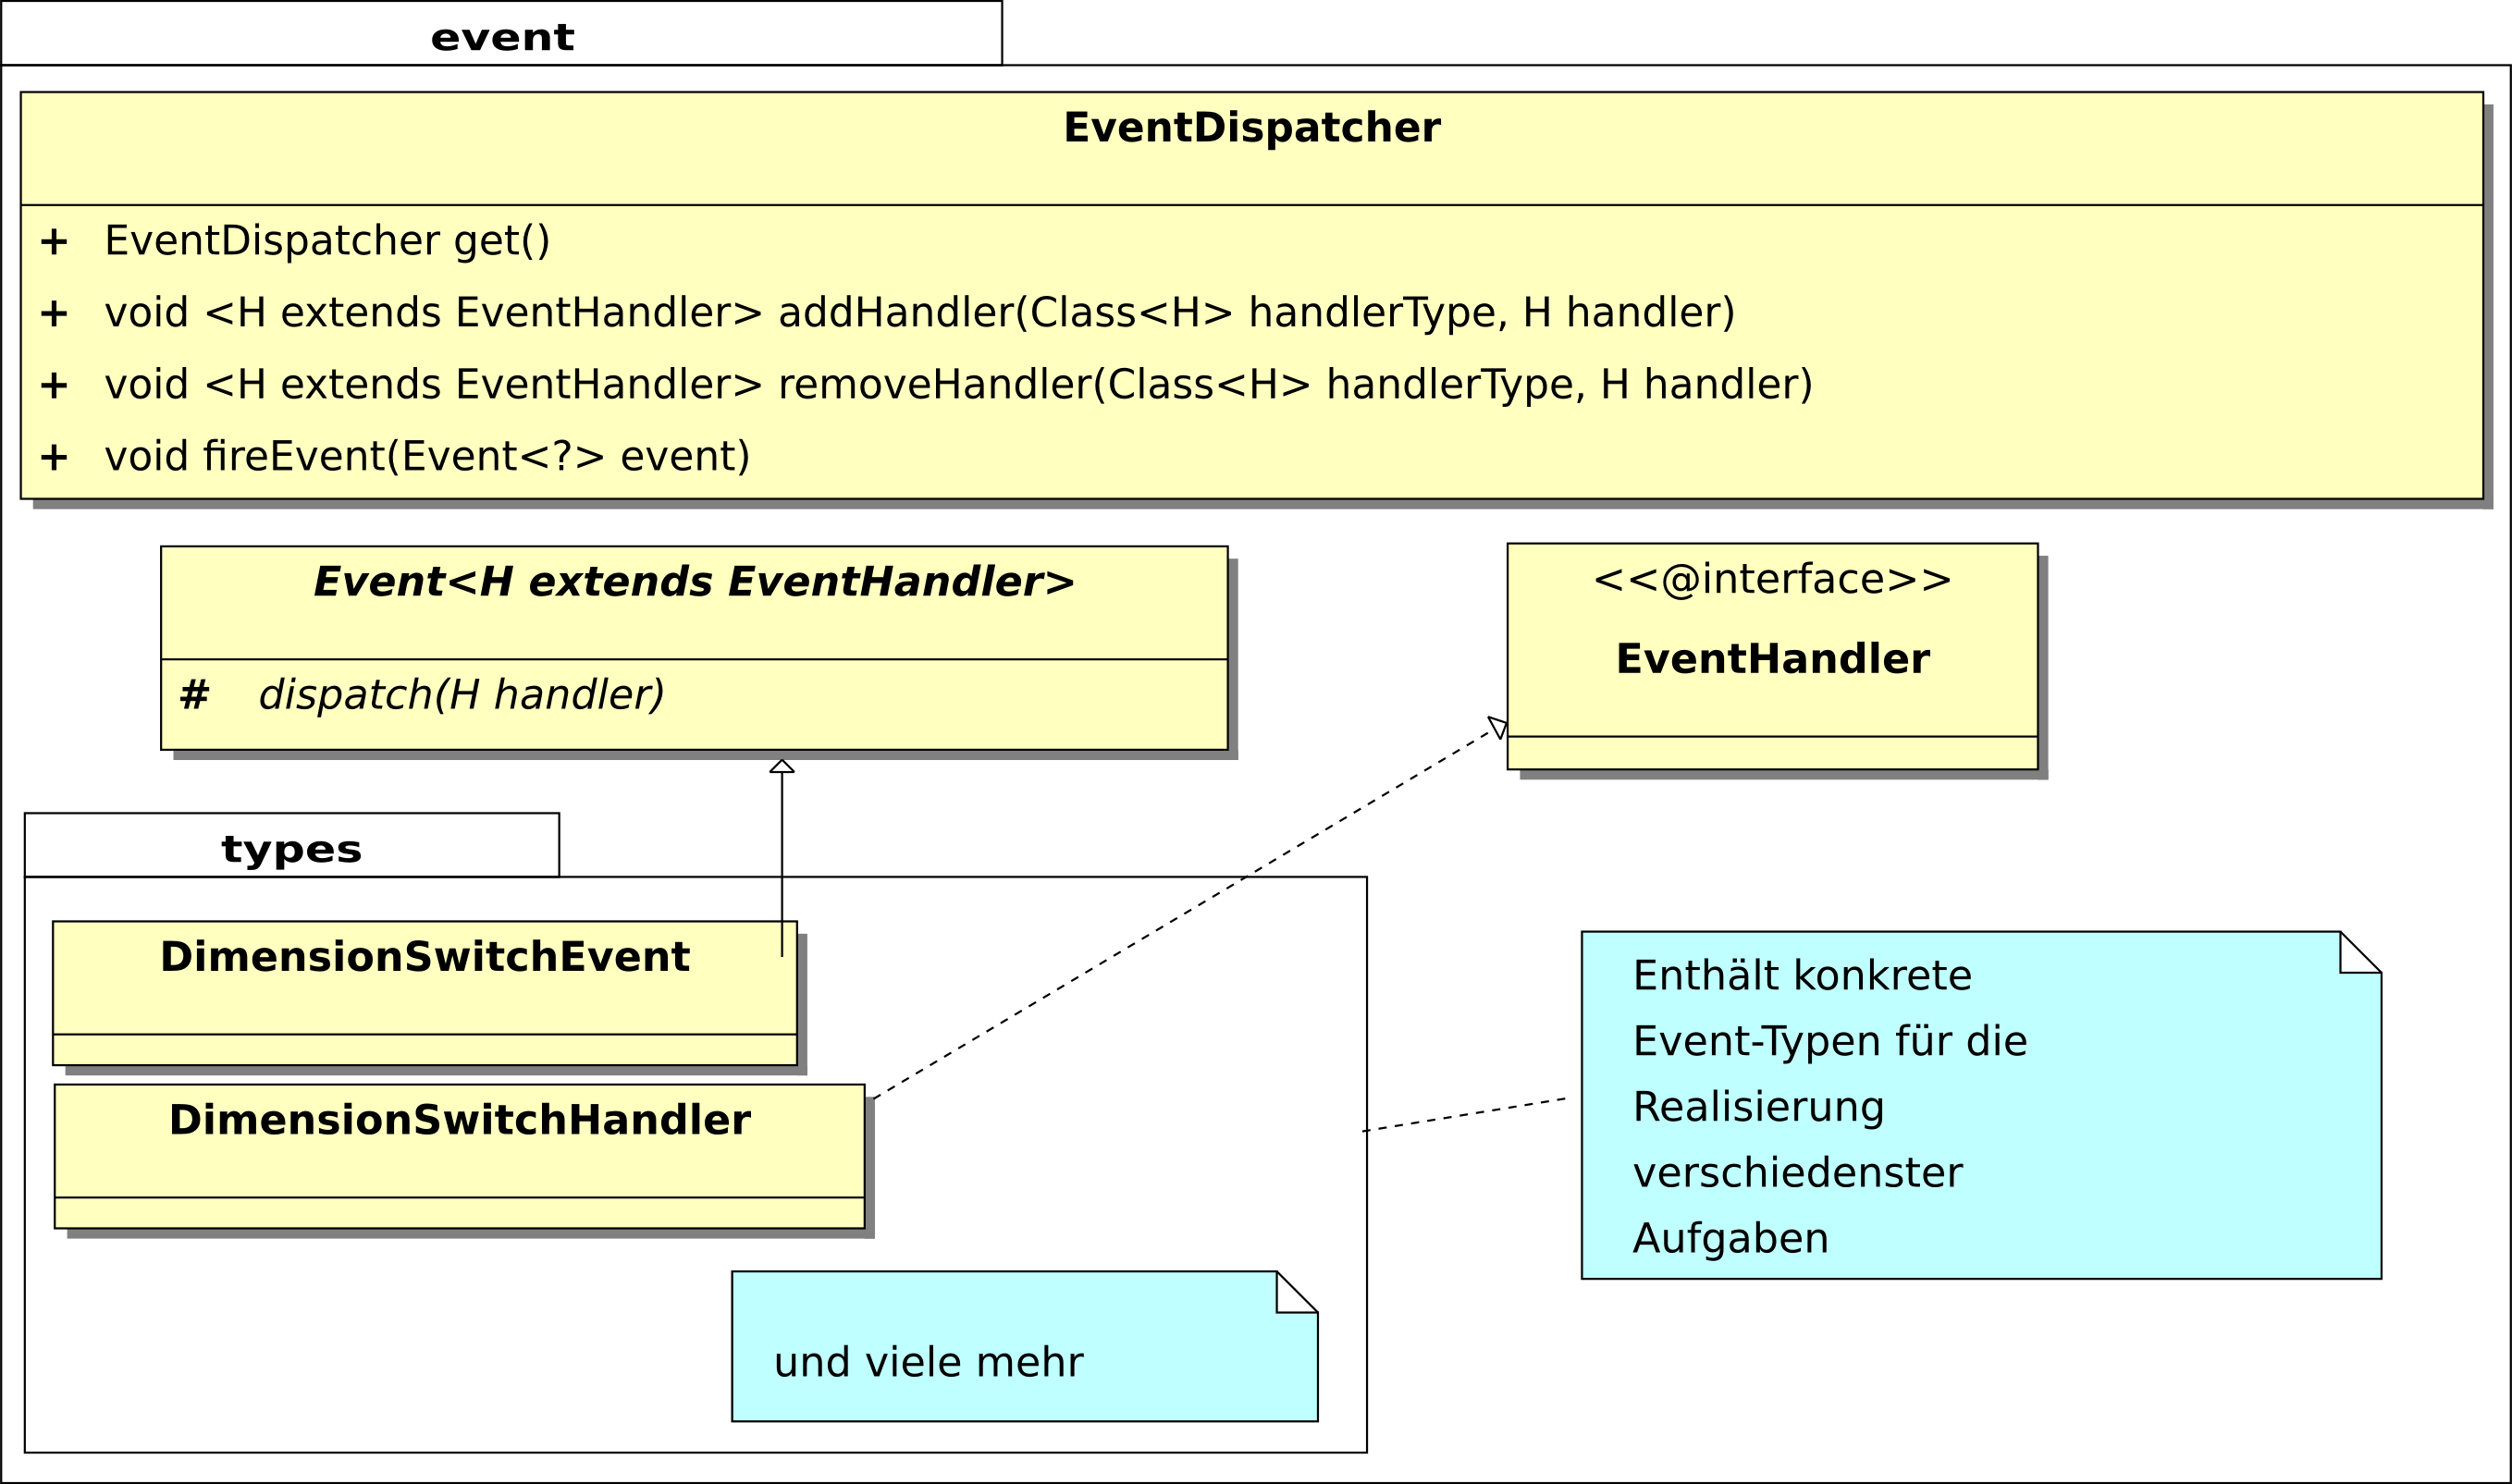
\includegraphics[width=0.8\textwidth]{img/event_classdiagram2}
            \caption{Klassendiagramm des Eventsystems}
        \end{figure}
        \subsubsection*{Events}
            Events sind konkrete Reaktionen auf bestimmte Ereignisse und enthalten je nach Ereignis entsprechende Kontextinformationen.
            Alle Typen von Events erben von der abstrakten Klasse \lstinline|Event<H extends EventHandler>| und stellen einen
            zugehörigen \lstinline|EventHandler|-Typen bereit.
            Komponenten, die auf ein bestimmtes Event reagieren sollen, realisieren das zum Event zugeordnete
            \lstinline|EventHandler|-Interface und implementieren damit eine Reaktionsmethode mit komponentenspezifischem
            Code.

            Eine zentrale Singleton-Instanz, der \lstinline|EventDispatcher|, koordiniert dann das Absenden und Empfangen von Events
            und verteilt die Ereignismeldungen an Interessenten.
            Hierfür muss jede an einem spezifischen Event interessierte Komponente sich als solche beim
            \lstinline|EventDispatcher| registrieren (\lstinline|addHandler(Class<H> eventType, H handler)|).
            Eine designierte Eventquelle hält ebenfalls einen Verweis, um mittels dessen
            \lstinline|fireEvent(Event<?> e)|-Methode im Zuge einer Reaktion ein Event abzufeuern.

      %  \subsubsection*{Eventimplementierung}
      %      Event-Typen werden durch Anlegen einer Event-Klasse und einer EventHandler-Klasse hinzugefügt.%
%
%            Das EventHandler-Template ist
%            
%            \begin{code}
%                import pointGroups.gui.event.EventHandler;
%
%                public interface ConcreteHandler
%                    extends EventHandler
%                {
%                    public void onConcreteEvent(final ConcreteEvent event);
%                }
%            \end{code}
%
%            Das Event-Typ-Template ist
%
%            \begin{code}            
%                import pointGroups.gui.event.Event;
%
%                public class ConcreteEvent
%                    extends Event<ConcreteHandler>
%                {
%                    public final static Class<ConcreteHandler> TYPE =
%                        ConcreteHandler.class;
%
%                    @Override
%                    public final Class<ConcreteHandler> getType() {
%                        return TYPE;
%                    }
%
%                    @Override
%                    protected void dispatch(final ConcreteHandler handler) {
%                        handler.onConcreteEvent(this);
%                    }
%                } 
%            \end{code}
%            
%            wobei Concrete durch konkrete Namen ersetzt werden kann.
            
        \subsubsection{GUI\label{ssec:gui}}

            Für die Darstellungen der geometrischen Objekte wird die Bibliothek
            jReality~\cite{jreality} benutzt.
            %, welche unteranderem mehrere 3D- Backends
            %unterstützt, wobei in diesem Projekt OpenGL als Standard- Backend
            %verwendet wird.
            jReality wird von der TU-Berlin entwickelt, steht unter der BSD-
            Lizenz und ist quelloffen, frei verwendbar und anpassbar.

            Eigentlich ist jReality eine umfangreiche Ansammlung von Werkzeugen,
            welche sich nicht nur auf das Anzeigen von geometrischen Objekten
            beschränkt und dadurch z.B. auch eine eigene Oberfläche für die Nutzung
            dieser Werkzeuge bereitstellt.

            \noindent Jedoch wurden diese zusätzlichen Features für das Projekt nicht
            gebraucht und daher die mit angebotene Oberfläche nicht genutzt. jReality
            bietet die Möglichkeit, nur das Render-Fenster, also das Fenster wo
            die Objekte angezeigt werden, zu verwenden und dieses 
            nahtlos als Swing-Unterkomponente in die GUI einzubinden.

            %Um geometrische Objekte in jReality zeichnen zu können, muss dieses
            %Objekt in ein von jReality verständliches Format gebracht werden.

            Es werden zwei jReality-Instanzen benutzt, wobei die eine den
            Fundamentalbereich und die andere das Schlegeldiagramm zeichnet.

            \noindent Ansonsten gibt es in der GUI Steuerungselemente, um den
            Fundamentalbereich bzw. das Schlegeldiagramm berechnen zu können.
            Außerdem wurde eine Liste der Punktgruppen aus 3D bzw. 4D eingebaut um
            aus diesen zu wählen.

\subsection{Implementierung von Berechnungen}
    \subsubsection{Symmetriebilder}
        Wie bereits in Abschnitt~\ref{ssec:quad3sym} beschrieben, können Elemente der Symmetriegruppen (Drehungen, Spiegelungen) als Quaternionen beschrieben werden.
        Das Bild eines Punktes $p$ bezüglich einer Drehung bzw. einer Spiegelung kann dann durch einfache Multiplikationsoperationen berechnet werden.
        Der Algorithmus~\ref{alg:images} zeigt einen einfachen Pseudocode, der bei Eingabe eines Punktes $p$ und einer Symmetriegruppe $sym$ alle Bilder von $p$ berechnet.

        \begin{lstlisting}[mathescape, morekeywords={for, each, do, begin,input, output, end, return}, caption={Peusdocode der Bildmengenberechnung}, label=alg:images]
    input: sym = {s$_1$, ..., s$_n$}: Symmetry group
           p: Point
    output: images: All images of p with respect to sym
    
    begin
        images $\gets$ {}
        for each s $\in$ sym do
            q $\gets$ rotate p according to s
            images $\gets$ images $\cup$ {q}
        end
    end
        \end{lstlisting}
    \subsubsection{Symmetriegruppen}
    Eine Symmetriegruppe wird durch einen Enum repräsentiert. Durch diesen Enum wird auf Hashmaps zugegriffen. Es gibt jeweils eine Hashmap für die Gruppenelemente und die Untergruppen. Dies erleichtert das Hinzufügen von Symmetriegruppen, deren Zugriff und die Verwaltung von Gruppenelementen. Es ist im Gegensatz zu unserem ursprünglichen Entwurf nur eine Klasse für den dreidimensionalen Fall nötig und es gibt deutlich weniger Redundanzen. Dies betrifft insbesondere die Nutzung von Gruppenelementen und die Untergruppenbeziehungen. Dieser Entwurf ist somit leichter wartbarer und wiederbenutzbarer.
    Für die Nutzung der Symmetriegruppen steht ein Interface bereit, welches einen leichten und intuitiven Zugang ermöglicht. Die wesentlichen Funktionen sind die Ausgabe der verschiedenen Bezeichnungen einer Gruppe, die Ordnung, die Untergruppen und die Berechnung der Punktgruppe zu einem gegebenen Punkt. Dies war besonders beim Entwurfswechsel sinnvoll. Denn so musste im restlichen Quellcode beim Entwurfswechsel nur sehr wenige Änderungen vorgenommen werden. Dieses Interface wird sowohl für den dreidimensionalen Fall sowie für den vierdimensionalen Fall verwendet.\\ 
%% 3D case
    Die dreidimensionalen Symmetriegruppen sind ausgiebig dokumentiert und nicht sehr umfangreich im Vergleich zum vierdimensionalen Fall. Wir konnten dort die Gruppenelemente als auch die Untergruppen festkodieren. Die Rotationsachsen wurden als statische Variablen gespeichert. Die einzelnen Gruppen werden dann durch diese Auswahl der Rotationsachsen charakterisiert. Die Rotationsachsen werden als Quaternionen dargestellt. \\
%%%% 4D-case
Im vierdimensionalen Fall waren die Symmetriegruppen in der Literatur nur durch die Generatoren beschrieben und eine händische oder halbautomatische Erzeugung erscheint bei den Gruppengröße von teilweise einigen tausend Elementen nicht sinnvoll. Wir haben uns dazu für die Erzeugung mittels Gruppen entschieden. Dies ist nachträglich für den dreidimensionalen Fall auch möglich und die Ergebnisse wurden in diesem Fall auch verifiziert. Im vierdimensionalen Fall haben wir die Klassen Symmetrie4D, Symmetry4DReflection, Rotation4D, Reflection4D und SubgroupChecker4D.
Symmetry4D ist analog zu Symmetry3D aufgebaut. Es werden allerdings die Gruppen mittels Hintereinanderausführen der Generatoren bestimmt und die neuen Elemente werden gespeichert beziehungsweise geladen.
\begin{lstlisting}[mathescape, morekeywords={for, each, if, then, fi, do, begin,input, output, end, return}, caption={Peusdocode der Symmetriegruppeerzeugung}, label=alg:fromgen]
input: gen = {(l$_1$,r$_1$),...,(l$_n$,r$_n$)}: Generators
output: sym: Symmetry group
begin	
	sym $\gets$ gen
	newElem $\gets$ false
	do
		for each (l$_i$,r$_i$) $\in$ sym do
			for each (l$_j$,r$_j$) $\in$ sym do
				e $\gets $ (l$_i \cdot$ l$_j$, r$_i \cdot$r$_j$)
				if (e $\notin$ sym) then
					sym $\gets$ sym $\cup$ {e}
					newElem $\gets$ true
				fi
			end
		end
	while (newElem)
end 

\end{lstlisting}
Das Hauptproblem dabei ist das Überprüfen, ob ein Element bereits in einer Gruppe vorhanden ist. Bei Gruppen von mehreren tausend Elementen ist eine naive Suche zu zeitintensiv und es kann zu Rundungsfehlern kommen. Aus diesem Grund haben wir uns für eine Hashmap zur Speicherung der Elemente entschieden. Dazu mussten für eine Rotation eine Hashmethode erzeugt werden. Die wichtigen Anforderungen an die Hashmethode für unseren Entwurf waren eine effiziente Berechnung, im Einklang mit einer equal-Methode und eine gute Streuung der Elemente.\\
Für das Hashen von Quaternionen haben wir uns an eine Implementierung von JReality orientiert. Mit den Hash- und Equal-Methoden wird gleichzeitig, dass Problem von Rundungsfehler gelöst. Wir runden auf fünf Nachkommastellen und bilden somit ein Gitter. 
\begin{lstlisting}[mathescape, morekeywords={for, each, if, then, fi, do, begin,input, output, end, return}, caption={Peusdocode der Erzeugung von Hashcode eines Quaternions}, label=alg:hash]
input: q = (re,i,j,k): Quaternion
output: hashcode: int
begin	
	r $\gets 10^5$
	x = round(r$\cdot$re) / r
    	y = round(r$\cdot$i) / r
    	z = round(r$\cdot$j) / r
    	w = round(r$\cdot$k) / r
	hashcode $\gets$ 31$\cdot$hashcode + x$\oplus$x
	hashcode $\gets$ 31$\cdot$hashcode + y$\oplus$y
	hashcode $\gets$ 31$\cdot$hashcode + z$\oplus$z
	hashcode $\gets$ 31$\cdot$hashcode + w$\oplus$w
end 
\end{lstlisting}
In Rotation4D wird eine Rotation mittels zwei Quaternionen dargestellt und ein Punkt kann mit der Methode gemäß der mathematischen Definition rotiert werden. Als Hashcodefunktion werden die beiden Hashwerte der Quaternionen mit einem XOR verknüpft. Nach ~\cite{conway2003} gelten folgenden Gleichheiten
$[-l,-r] = [l,r]$ und $[-l,r]=[l,-r]=-[l,r]$. Damit der Hashcode mit den Gleichheiten im Einklang steht, werden negative Quaternionen beim Hashen zu positiven transformiert. Beim Gleichheitstest werden jeweils die einzelnen Quaternionen verglichen.\\
Die Erzeugung der Rotationsgruppen ist sehr zeitintensiv. Aus diesem Grund werden die Rotationsgruppen im vierdimensionalen Fall mittels Java-ObjectOutputStream jeweils in eine Datei gespeichert und von dort geladen. Sollten die Dateien nicht gefunden werden, so werden die Rotationsgruppen erzeugt und lokal gespeichert. Die erzeugten Gruppen wurden mittels JUnittest überprüft. Dazu wurde jeweils die Gruppengröße der erzeugten Gruppe mit der angegebenen Gruppengröße in der Literatur verglichen. Die Untergruppenbeziehungen wurden mittels naivem Test untersucht. Dazu wurden überprüft, welche Gruppe in einer anderen Gruppe enthalten ist.\\
Für vierdimensionale Gruppen mit Spiegelungen werden in die Rotationsgruppen erweitert. Bei der Berechnung der Bilder werden dazu zu nächst alle Bilder unter Rotationen bestimmt. Anschließend werden diese Bilder noch mit dem entsprechenden Quaternion erweitert.
\begin{lstlisting}[mathescape, morekeywords={for, each, if, then, fi, do, begin,input, output, end, return}, caption={Peusdocode für Bilder unter Spiegelungen}, label=alg:images2]
input: e = (re,i,j,k): Quaternion // extending element
	 rotations = (q$_1$,..q$_n$): All rotions of given point p with respect to rotationsym
	
output: images: All images of p with respect to sym
begin	
	images $\gets$ rotations
	for each q $\in$ rotations do
		images $\gets$ images $\cup$ reflect(e,q)
	end
end 
\end{lstlisting}
Die Untergruppenbeziehungen konnten aus den Rotationsgruppen übernommen werden, wenn das gleiche Quaternion zur Erweiterung genommen wurde.
\\ \todo{Umsortieren}
  \todo{Formulierung?}


    \subsubsection{Fundamentalbereich}
         In Abschnitt \ref{fundamentalbereich} wurde in Definition \ref{fundamentalbereich:voronoi} der Voronoi-Fundamentalbereich beschrieben. Zur Berechnung der Punktgruppen soll eine dieser Zellen ausgewählt und visualisiert werden.
         Zur einfacheren Darstellung eines Abschnitts der Sphäre $S^3$ berechnen wir zunächst die Projektion des Voronoi--Fundamentalbereichs auf eine $\mathbb{R}^3$ Ebene.
        \subsubsection*{Idee}
            Wir lassen zunächst die Symmetriegruppe auf ein ausgezeichnetes Element $x$ wirken.

            \noindent Als erstes Berechnen wir die Voronoi--Zelle für $x$ bezüglich des Orbits von $x$. Alle Punkte die innerhalb dieser Voronoi--Zelle liegen, sind Elemente von $S^3$. 
            Da die Gruppe symmetrisch ist, können wir nicht zwei Elemente aus dem selben Orbit haben. 
            Andernfalls müsste ein zweiter Punkt näher an einem anderen Element aus $G \rhd x$ liegen.
            Dabei ist es notwendig, dass sich der Punkt $x$ nicht auf einer Rotationsachse oder Spiegelebene befindet, da sonst die Voronoi--Zellen zu groß ausfallen.
            
            Anschließend projizieren wir diese Zelle auf eine Ebene, die tangential auf dem Kugelsegment liegt. Dazu wählen wir die Ebene $h \, : \, [t - x] \cdot x = 0$ in Normalendarstellung, da wir wissen, dass $x$ auf der Kugeloberfläche im Kreissegment liegt und $x$ auch ein Normalenvektor ist.
            
        \subsubsection*{Umsetzung}
         Eine Voronoi--Zelle von $x$ für eine Menge von Zentren $S$ ist definiert als 
         $$ VC(x) = \bigcap_{s \in S \setminus \{ x \}} h^+_{x,s}$$
         Wobei $h^+_{x,s}$ der Halbraum ist, der rechts von der Hyperebene liegt, die zu $x$ und $y$ in jedem Punkt den selben Abstand hat.\\
         
         \noindent In polymake kann die Voronoi--Zelle als Polytop über den Schnitt von den zugehörigen Halbräumen definiert werden. Dies geht über den Befehl

         \begin{code}
            new Polytope(INEQUALITIES=>\$hyperplanes)
         \end{code}

         Dabei ist \$hyperplanes eine Menge von Hyperebenen. Falls ein affines Polytop vorliegt, wie in unserem Fall in der Ebene $h$, die wie im letzten Abschnitt
         definiert ist, können wir auch dies mit in die Erzeugung mittels

         \begin{code}
new Polytope(INEQUALITIES=>\$hyperplanes, EQUATIONS=>{h})
         \end{code}

         eingeben und haben so $VC(x)$ berechnet. \todo{Wieso wird die Ebene mit eingegeben?}
         
         \noindent Das Polytop befindet sich nun in der Ebene. Für die Darstellung in $n-1$ Dimensionen berechnen wir nun eine geeignete Basis, so dass die Eckpunkte des Polytops durch $n-1$ Koordinaten darstellen werden können. 
         Der Punkt $x$ steht senkrecht auf der Ebene und ist damit für die Darstellung 
         unerheblich. Wir berechnen eine Orthonormalbasis für die Ebene mit $x$ als erstem Basisvektor. Nun können wir leicht eine Basiswechselmatrix angeben,
         da die Bilder der neuen in der alten Basis bekannt. Darüber hinaus ist diese Matrix orthogonal -- da die Spalten eine Orthogonalbasis waren, weshalb die zu diesem Basiswechsel inverse Matrix durch Transponieren einfach ermittelt werden kann.

         Wir haben nun also zwei Matrizen, um beide Darstellungen ineinander umzurechnen. In der neuen Basis können wir nun die erste Komponente weg lassen, da diese nach der Projektion auf null abgebildet wird. Daraus resultiert eine Darstellung in $n-1$ Dimensionen.
         Beim Zurückrechnen muss nur beachtet werden, dass sich die Punkte in einer affinen Ebene mit Stützvektor $x$ befinden.

        \subsubsection*{Berechnung}

         Die Definition von Hyperebenen in polymake hat die Darstellung
         $$
            h \, : \, [a_0, ..., a_n] \rightsquigarrow a_0 + a_1 x_1 + \cdots + a_n x_n = 0
         $$
         und entsprechend für Halbräume mit $\geq 0$.\\

         \noindent Die Halbräume für unser Polytop genügen der Gleichung
         $$
            t \cdot (x - s) \geq 0 \Leftrightarrow 0 + (x_1-s_1)\cdot t_1 + \cdots + (x_n -s_n)t_n \geq 0,
         $$
         wobei $x$ der gewählte Vektor war und $s \not= x$ aus dem Orbit von $x$ stammt.

         \noindent Damit können wir alle Halbräume aus dem Orbit berechnen. Die affine Ebene genügt der Gleichung
         $$
            (t - x) \cdot x = 0 \Leftrightarrow - \left( \sum_{i=1}^n x_i^2 \right) + t_1 x_1 + \cdots t_n x_n = 0
         $$
         und kann auch leicht erstellt werden. Um das von uns gewünschte Polytop zu bekommen, benutzen wir das folgende polymake-Script

         \begin{code}
my \$poly = new Polytope(INEQUALITIES=>\$hyperplanes, EQUATIONS=>\$affine);
print \$poly->VERTICES;
print \$poly->EDGES;
print \$poly->FACETS;
         \end{code}

         \noindent Mit diesen Ergebnissen können wir nun die Basiswechselmatrizen berechnen und so die Punkte umrechnen. Das Objekt \emph{Fundamental} ist somit
         eine Sammlung dieser Eigenschaften.
         
\begin{lstlisting}[language=Java, caption={Auswahl aus dem Fundamental Interface}, label=fund:interface]
public interface Fundamental {
   public double[][] getVertices();
               
   public Edge<Integer,Integer>[] getEdges();

   public double[] revertPoint(double[] point);

   public boolean inFundamental(double[] point);
}
\end{lstlisting}
         
         \noindent Die ersten beiden Funktionen liefern entsprechend ihrer Namensgebung die Knoten und Kanten des Fundamentalbereichs. Die dritte Methode \emph{revertPoint} nimmt einen Punkt in $\mathbb{R}^{n-1}$ und
         hebt ihn auf die Oberfläche der $S^{n-1}$ zurück. Die letzte Methode überprüft, ob ein angegebener Punkt überhaupt in der Voronoi--Zelle liegt.
         Diese Methode wird bei der Anzeige benötigt, um bei der Punktauswahl keine Punkte außerhalb das Polytops auszuwählen.\\

         \noindent Das Ganze ist eine Schnittstelle, da wir als Fallback-case, falls die Berechnung das Fundamentalbereichs einmal fehl schlägt, immer noch 
         den Bereich $S^{n-2}$ benutzen können. Dies ist kein Fundamentalbereich, da wir alle Orbits mehrfach treffen. Allerdings werden wir, außer im Falle
         der Identität, jeden Orbit mindestens einmal treffen.


